\svnid{$Id: ds_background.tex 1 2015-08-30 15:39:28Z mooiman $}

\chapter{Background}
\label{chap:ds_background}

\section{About the framework}
\label{sec:aboutdeltashell}

The framework will be gradually extended to allow for the integration of a variety of environmental models.

The framework is an integrated modeling environment to provide users with a single application which acts as a platform to integrate various locations and failure mechanisms. This is achieved by making use of a software framework specifically focused to provide a set of components which can be reused by all kinds of models. The overall picture of what functionality needs to be provided has been proposed by a variety of (potential) users and has been captured in so-called user stories. These user stories have been gathered in a so-called mind map which is presented in \Fref{Fig:MindMapUserStories}.
\begin{figure}[!ht]
\center
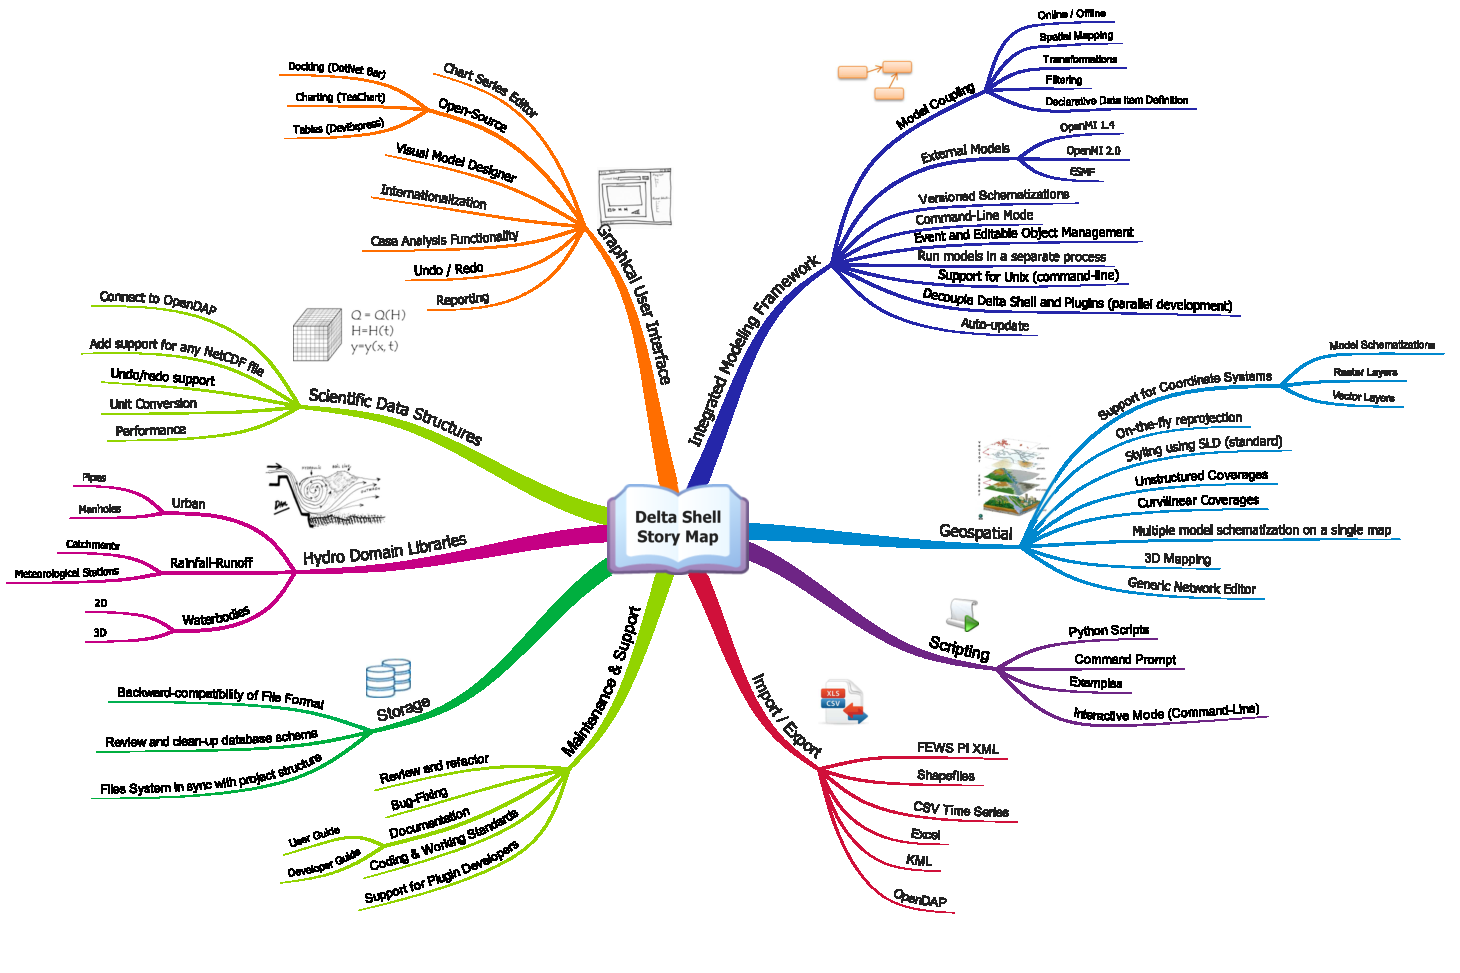
\includegraphics[width=\textwidth]{Figures/Chapter_background/DeltaShellStoryMap.pdf}
\caption{NEEDS TO BE UPDATED / REMOVED: Mindmap with key user stories.}
\label{Fig:MindMapUserStories}
\end{figure}
As can be seen from the mind map, the framework has to comply with a broad range of wishes defined by various users and user groups. Main topics (depicted in the main branches) are: 
\begin{itemize}
\item The definition of the integrated modeling framework, 
\item Data management: structuring, importing/exporting, storage.
\item Dealing with environmental domain libraries (hydro, geo).
\item Application interfaces (APIs) such as a graphical user interface or a command line interface using scripts for batch operation.
\item Documentation and support 
\end{itemize}
%
The framework provides a user-friendly and open environment for different locations and failure mechanisms. \Fref{fig:figstructure} shows the principles of the framework. It allows to combine different failure mechanisms (plug-ins), such as piping,  asphalt revetments, or macrostability. In this fashion, it is possible to compose various dedicated software suites within a single framework while preserving the same look-and-feel at the same time. Furthermore, common plug-ins with generic functionality may be used by all model plug-ins that have been integrated within the framework. Finally, tools for setting up or importing different types of data, perform calculations of the different failure mechanisms or combinations of them, and analyse model results.
%
\begin{figure} [H]
	\centering
		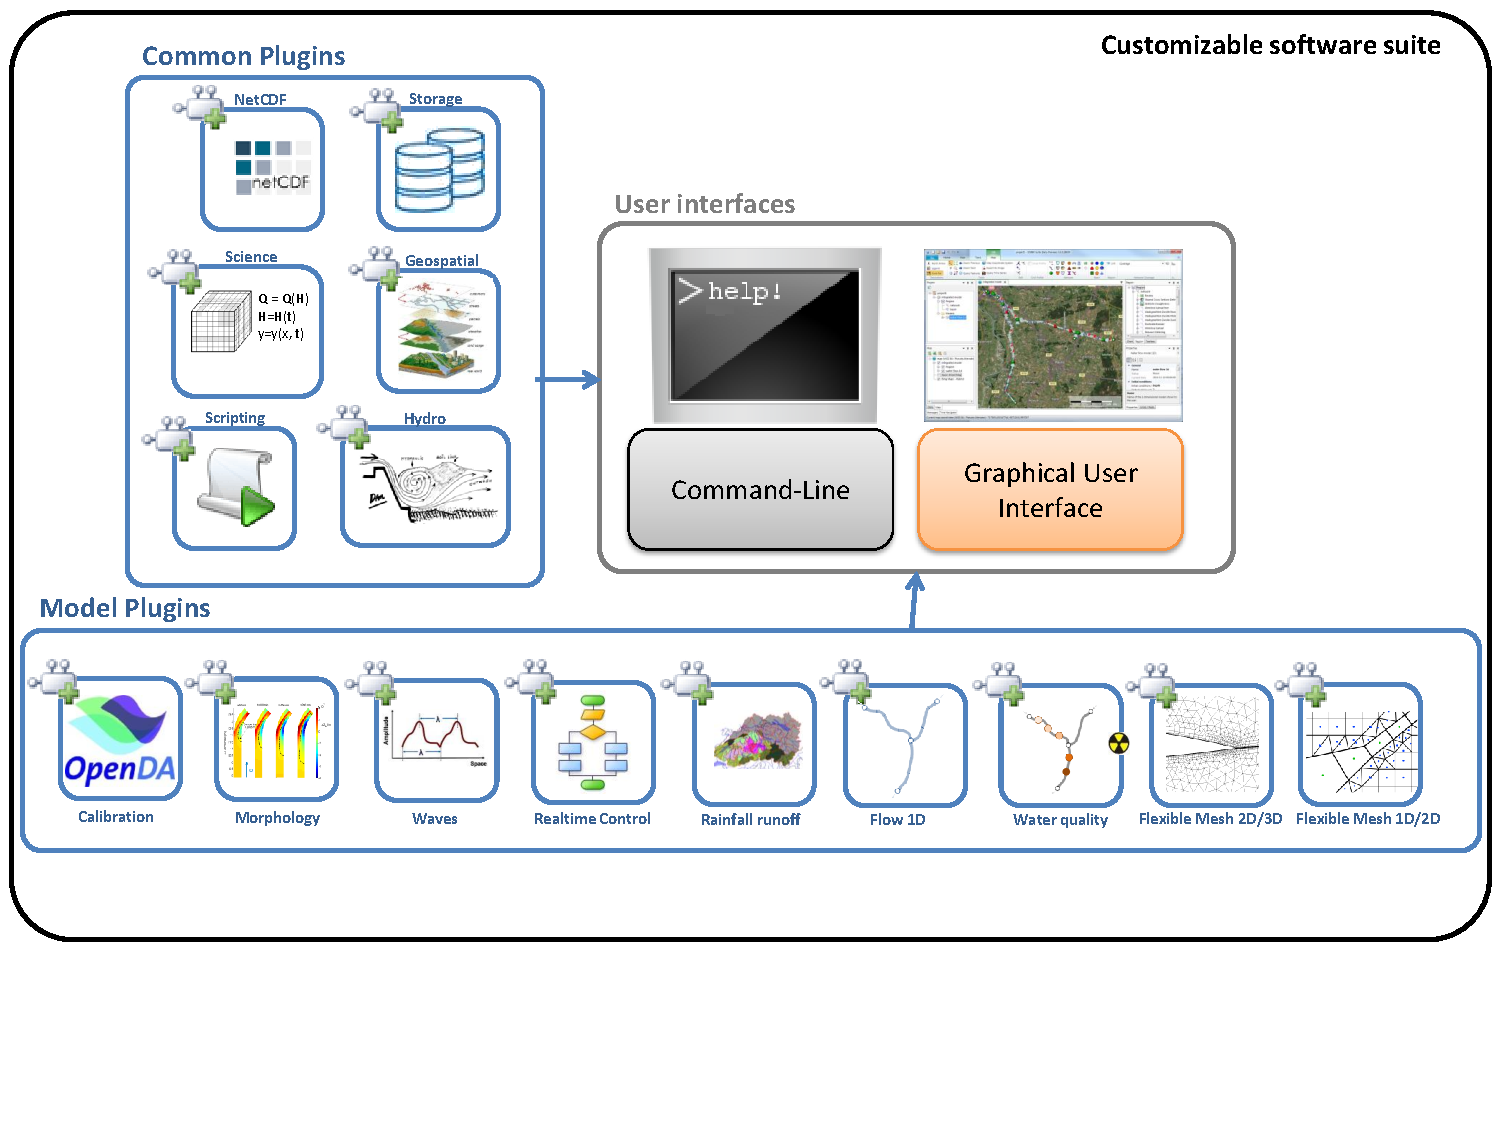
\includegraphics[width=\textwidth]{Figures/Chapter_overview/delta_shell_structure}
	\caption{The structure of DeltaShell  as integrated modelling suite.}
	\label{fig:figstructure}
\end{figure}

A model is, by definition, a simplified version of (a possible) reality. A generic model is a mathematical description of physical processes provided as a computer program. In combination with data for a specific part of the world, the model becomes a site-specific model. Within a site-specific model a set of boundary conditions forms a scenario.

The framework follows a layered concept to get from `real world' to `numerical model result' (\Fref{fig:fig2.0}).
Real objects usually are available on maps or other (digital) format.
Based on such data, the framework helps to create a schematisation, i.e.\ a network with model objects that correspond to the real objects.
The schematisation makes the model site-specific.
This model can be run under different sets of boundary conditions (scenarios).
Numerical solution of the equations with a failure mechanism plugin finally produces model results.
%
\begin{figure} [H]
	\centering
		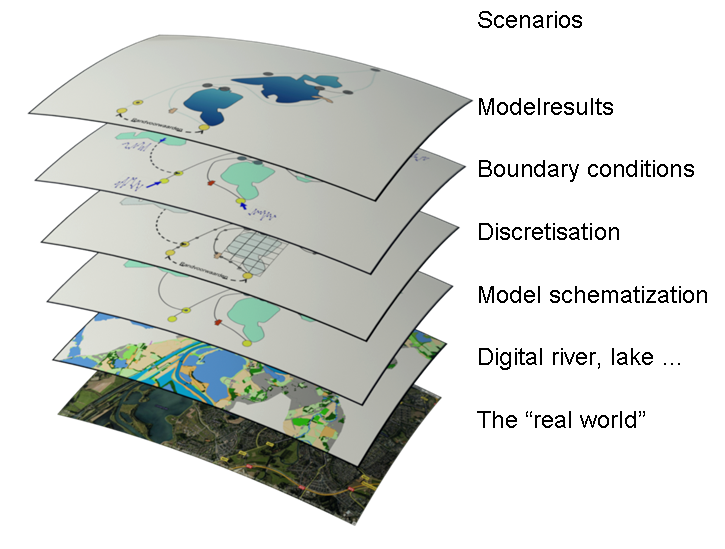
\includegraphics[width=\textwidth]{Figures/Chapter_background/DeltaShell_layers}
	\caption{TO BE UPDATED: From real world to model results.}
	\label{fig:fig2.0}
\end{figure}

\section{Framework: Vision Statement}
\label{sec:vision}
\textbf{For users:}\\
The framework should facilitate modelers in: schematization (with/without user interface), running tests in standardized modelling environments, batch execution (from command line) and parallel execution (on clusters). All modellers should be able to use the Framework combined with the failure mechanisms of their preference (piping, macrostability, etc.). \\\\
\textbf{For developers:}\\
The Framework should provide a generic, transparent and simple way of developing new or combining existing failure mechanisms (plug-ins). The emphasis should be on reuse and expansion of existing code and features.   

\section{Overall Architecture}
\label{sec:overallarchitecture}

This section gives an overview of the framework architecture and a description of its main components. The framework has been designed using a flexible architecture which can easily facilitate the use of external applications. The concept of the overall architecture is similar to existing commercial products like Eclipse or Microsoft Visual Studio Shell.
The most important subjects considering the architecture of Delta Shell are presented in \Fref{Fig:MindMapArch}. These are the subjects that need to come together within the architecture of the framework.

\begin{figure}[!ht]
\centering
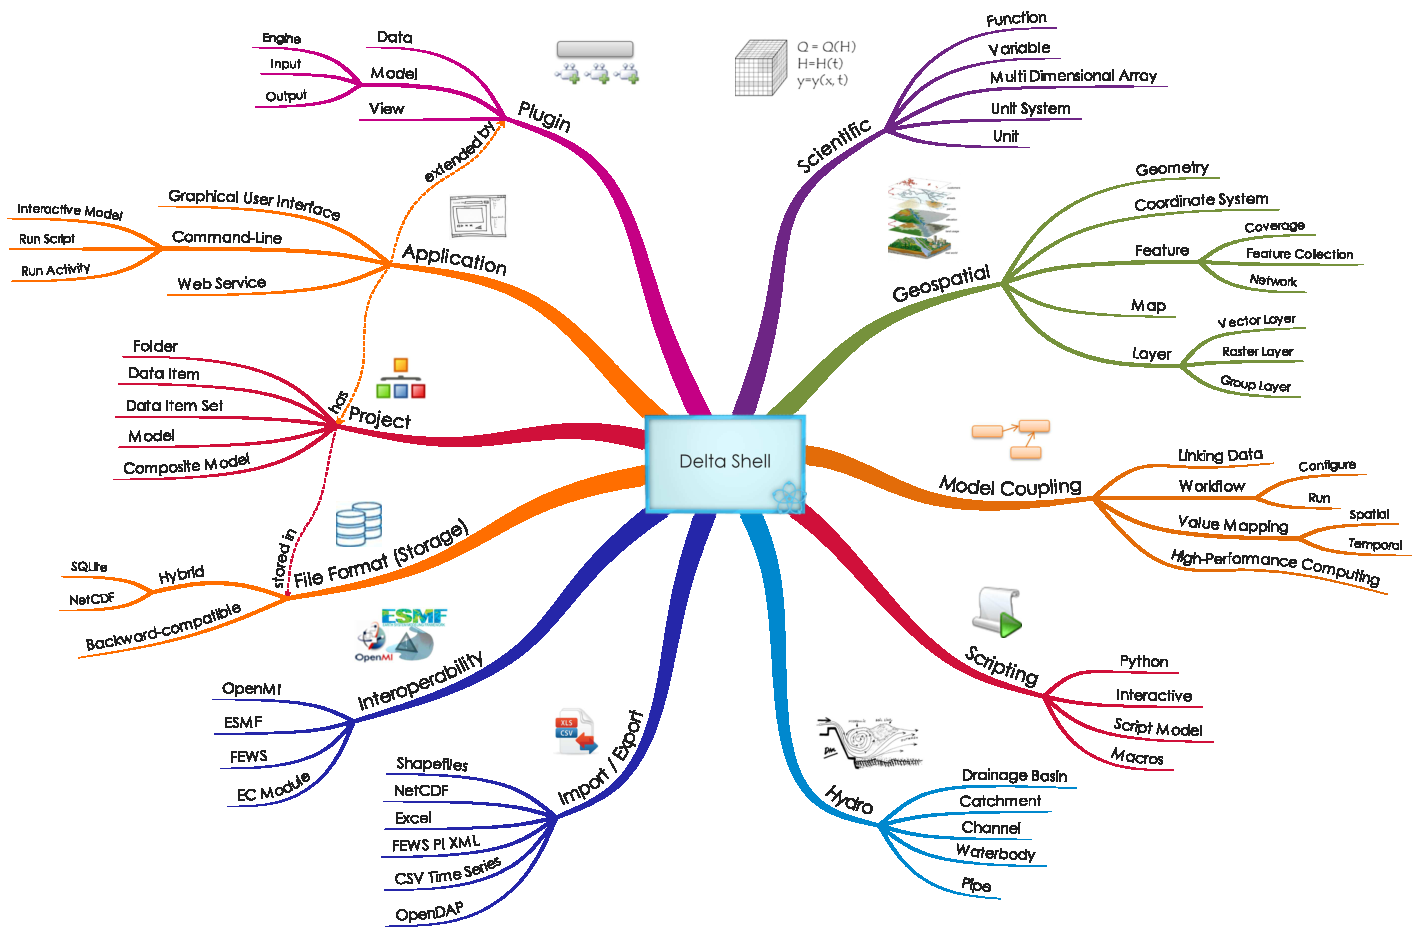
\includegraphics[width=\textwidth]{Figures/Chapter_background/ArchitectureMindMap.pdf}
\caption{TO BE UPDATED: Mindmap with key architecture subjects of Delta Shell.}
\label{Fig:MindMapArch}
\end{figure}


TO BE CONTINUED